\documentclass[12pt]{article}

% ---------- Packages ----------
\usepackage[margin=1in]{geometry}
\usepackage{amsmath,amssymb}
\usepackage{siunitx}        % units & numbers
\usepackage{booktabs}       % tables
\usepackage{caption}
\usepackage{subcaption}
\usepackage{graphicx}
\usepackage{float}
\usepackage{hyperref}
\usepackage{physics}
\usepackage{enumitem}
\sisetup{separate-uncertainty=true,detect-weight=true,detect-inline-weight=math}

% ---------- Title ----------
\title{Lab 1: Coulomb's Law}
\author{Zemon Xiao}
\date{22/09/2025}

\begin{document}
\maketitle

\begin{abstract}
We used a torsion balance to investigate Coulomb's Law for two charged conducting spheres. By changing the center--to--center separation we studied the distance dependence, and by changing the charging voltage at fixed separation we studied the charge dependence. The torsion angle was related to force through the balance's torsion constant. Parts A and B yielded repeatable datasets supporting the inverse--square law and linearity with charge; Part~C could not be finished due to equipment/time limits, so we provide a simulated calibration to illustrate how one would extract the torsion constant and Coulomb's constant.
\end{abstract}

% ---------- Theory ----------
\section*{Theory}
Coulomb's law for point charges reads
\begin{equation}
F = k\,\frac{q_1q_2}{R^2},
\end{equation}
where $F$ is the magnitude of the electrostatic force, $q_1$ and $q_2$ are the charges, $R$ is the \emph{center--to--center} separation, and $k$ is Coulomb's constant. In a torsion balance, the restoring torque of a thin wire is proportional to the angular displacement $\theta$; at equilibrium the electrostatic force equals the torsion force,
\begin{equation}
F = K_{\mathrm{tor}}\;\theta.
\end{equation}
Because our conductors are spheres, when $R$ is not much larger than the sphere radius $a$ the surface charge redistributes and reduces the force. The manual prescribes a finite--size correction factor
\begin{equation}
B = 1 - \frac{4a^3}{R^3},\qquad \theta_{\mathrm{corr}}=\frac{\theta}{B},
\end{equation}
with $a=\SI{1.9}{cm}$ for this apparatus. When we need a rough estimate of charge at a given voltage $V$, we use the capacitance of an isolated sphere, $C=4\pi\varepsilon_0 a$, and the approximation $q \approx C V$.

% ---------- Procedure ----------
\section*{Experimental Procedure}

The apparatus was set up on a stable bench away from drafts and direct sunlight. With the high-voltage supply turned off, both spheres and the torsion wire assembly were discharged to ground using the grounding lead. The base was leveled according to the manual so that the pointer could settle symmetrically. The zero mark on the scale was checked; the torsion knob was adjusted until the pointer coincided with the fiducial line and the reading was recorded as the mechanical zero. The radius of the conducting spheres was taken from the apparatus specification, \(a=\SI{1.9}{cm}\), for later finite-size corrections. Before any run we waited several seconds after touching the apparatus to allow charges induced by the operator to dissipate.

For the distance-dependence study (Part A) both spheres were first brought to the same polarity by briefly contacting them to the charging probe, then to each other, following the manual’s sequence to minimize contact electrification. The movable sphere was positioned using the slide’s center-to-center scale; the manual specifies that this scale already reads the separation between the sphere centers, so no further diameter correction was applied. A typical charging potential of \(6\!-\!7~\mathrm{kV}\) was used and kept constant throughout this part. At each programmed separation \(R=\{20,14,10,9,8,7,6,5\}\,\mathrm{cm}\), the movable sphere was approached slowly to avoid mechanical overshoot and air currents. After the electrostatic repulsion twisted the balance, the torsion knob was gently turned to bring the pointer back exactly to the reference line. The angle \(\theta\) indicated by the torsion dial was then read to the nearest degree once the pointer had settled (we allowed \(10\!-\!20~\mathrm{s}\) of damping). Three or more readings were taken at each \(R\) until the repeatability criterion of \(\pm 1^\circ\) was met; between separations the spheres were separated to more than \(25~\mathrm{cm}\) and discharged momentarily to reduce memory effects from residual charge. The order of \(R\) values was taken from large to small to reduce the chance of accidental contact between spheres, as recommended by the manual.

For the charge-dependence study (Part B) the center-to-center distance was fixed at \(R=\SI{9}{cm}\) using the same scale reference as in Part A. The supply voltage was then stepped through \(3,4,5,\) and \(6~\mathrm{kV}\) in ascending order. At each voltage, both spheres were first equalized to the new potential, the pointer was re-zeroed with the torsion knob, and a series of \(\theta\) readings was taken after waiting for the balance to settle. We again required at least three consistent readings within \(\pm 1^\circ\). If a slow drift of the pointer was observed at the higher voltages, the reading was taken as the time-average over several seconds, as suggested by the manual to mitigate leakage and air-current effects.

The final part (Part C) is a torsion-constant calibration intended to convert angles to forces. Following the manual’s guidance, a small known load is applied at the balance arm so that its weight \(W=mg\) produces a static torque that is balanced by the restoring torque of the wire; the torsion constant then follows from \(K_{\mathrm{tor}}\approx W/\theta\) (with \(\theta\) read in degrees when \(K_{\mathrm{tor}}\) is expressed in \(\mathrm{N/deg}\)). In our session, limitations of the equipment and time prevented a full calibration run. To illustrate the analysis, we therefore provide a short simulated calibration table in the Data Analysis section and use it only to demonstrate the calculation chain from \(K_{\mathrm{tor}}\) to the force \(F=K_{\mathrm{tor}}\theta_{\mathrm{corr}}\) and finally to \(k = F R^2/(q_1 q_2)\) when charges are estimated or measured. Throughout the experiment, we minimized systematics by discharging between runs, avoiding touching the spheres with bare hands, keeping sleeves and stationery away from the apparatus, and closing doors and windows to reduce air currents, in line with the manual’s recommendations.


% ============== DATA ANALYSIS ==============
\section*{Data Analysis}

\subsection*{Part A: Distance Dependence ($R$ varied, $V\approx 6$--$7$\,kV)}
Raw angles were corrected using $\theta_{\mathrm{corr}}=\theta/B$ with $a=\SI{1.9}{cm}$.
\begin{table}[H]
\centering
\caption{Part A raw angles and corrected quantities.}
\begin{tabular}{@{}rrrrr@{}}
\toprule
$R$ (cm) & $\theta$ (deg) & $B$ & $\theta_{\mathrm{corr}}$ (deg) & $1/R^2$ (cm$^{-2}$) \\
\midrule
20 & 5  & 0.9966 & 5.017 & 0.0025 \\
20 & 6  & 0.9966 & 6.021 & 0.0025 \\
20 & 7  & 0.9966 & 7.024 & 0.0025 \\
14 & 17 & 0.9900 & 17.172 & 0.0051 \\
14 & 15 & 0.9900 & 15.152 & 0.0051 \\
14 & 13 & 0.9900 & 13.131 & 0.0051 \\
10 & 26 & 0.9726 & 26.738 & 0.0100 \\
10 & 26 & 0.9726 & 26.738 & 0.0100 \\
10 & 27 & 0.9726 & 27.753 & 0.0100 \\
9  & 43 & 0.9624 & 44.700 & 0.0123 \\
9  & 42 & 0.9624 & 43.637 & 0.0123 \\
9  & 38 & 0.9624 & 39.480 & 0.0123 \\
8  & 52 & 0.9464 & 54.949 & 0.0156 \\
8  & 45 & 0.9464 & 47.555 & 0.0156 \\
8  & 51 & 0.9464 & 53.914 & 0.0156 \\
7  & 60 & 0.9200 & 65.217 & 0.0204 \\
7  & 59 & 0.9200 & 64.130 & 0.0204 \\
7  & 62 & 0.9200 & 67.391 & 0.0204 \\
6  & 65 & 0.8730 & 74.460 & 0.0278 \\
6  & 67 & 0.8730 & 76.762 & 0.0278 \\
6  & 67 & 0.8730 & 76.762 & 0.0278 \\
5  & 73 & 0.7805 & 93.571 & 0.0400 \\
5  & 76 & 0.7805 & 97.403 & 0.0400 \\
5  & 75 & 0.7805 & 96.059 & 0.0400 \\
\bottomrule
\end{tabular}
\end{table}

\paragraph{Formula.}
\[
\theta_{\mathrm{corr}}=\frac{\theta}{B},\qquad
B=1-\frac{4a^3}{R^3},\quad a=\SI{1.9}{cm}.
\]

\paragraph{One worked example.}
At $R=\SI{9}{cm}$, $B=1-4(1.9^3)/9^3\approx 0.9624$. For $\theta=42^\circ$,
$\theta_{\mathrm{corr}}=42/0.9624\approx 43.64^\circ$.

We then averaged the corrected angles at each $R$ and computed the sample standard deviation to quantify scatter. The per–$R$ means (used for plotting) are:
\[
\bar\theta_{\mathrm{corr}}=\{6.02,\,15.15,\,27.08,\,42.60,\,52.13,\,65.58,\,75.98,\,95.66\}^\circ
\quad\text{for }R=\{20,14,10,9,8,7,6,5\}\,\text{cm}.
\]

\paragraph{Plots and results.}
Figure~\ref{fig:partA_loglog} shows $\log\bar\theta_{\mathrm{corr}}$ vs.\ $\log R$ with a linear fit; the slope is $n=-2.035\ (\pm\ \text{fit})$, consistent with the inverse–square law.  
Figure~\ref{fig:partA_invR2} shows $\bar\theta_{\mathrm{corr}}$ vs.\ $1/R^2$ with a linear fit $y=(2426.78)\,x + 6.95$ and $R^2=0.952$.

\begin{figure}[H]
  \centering
  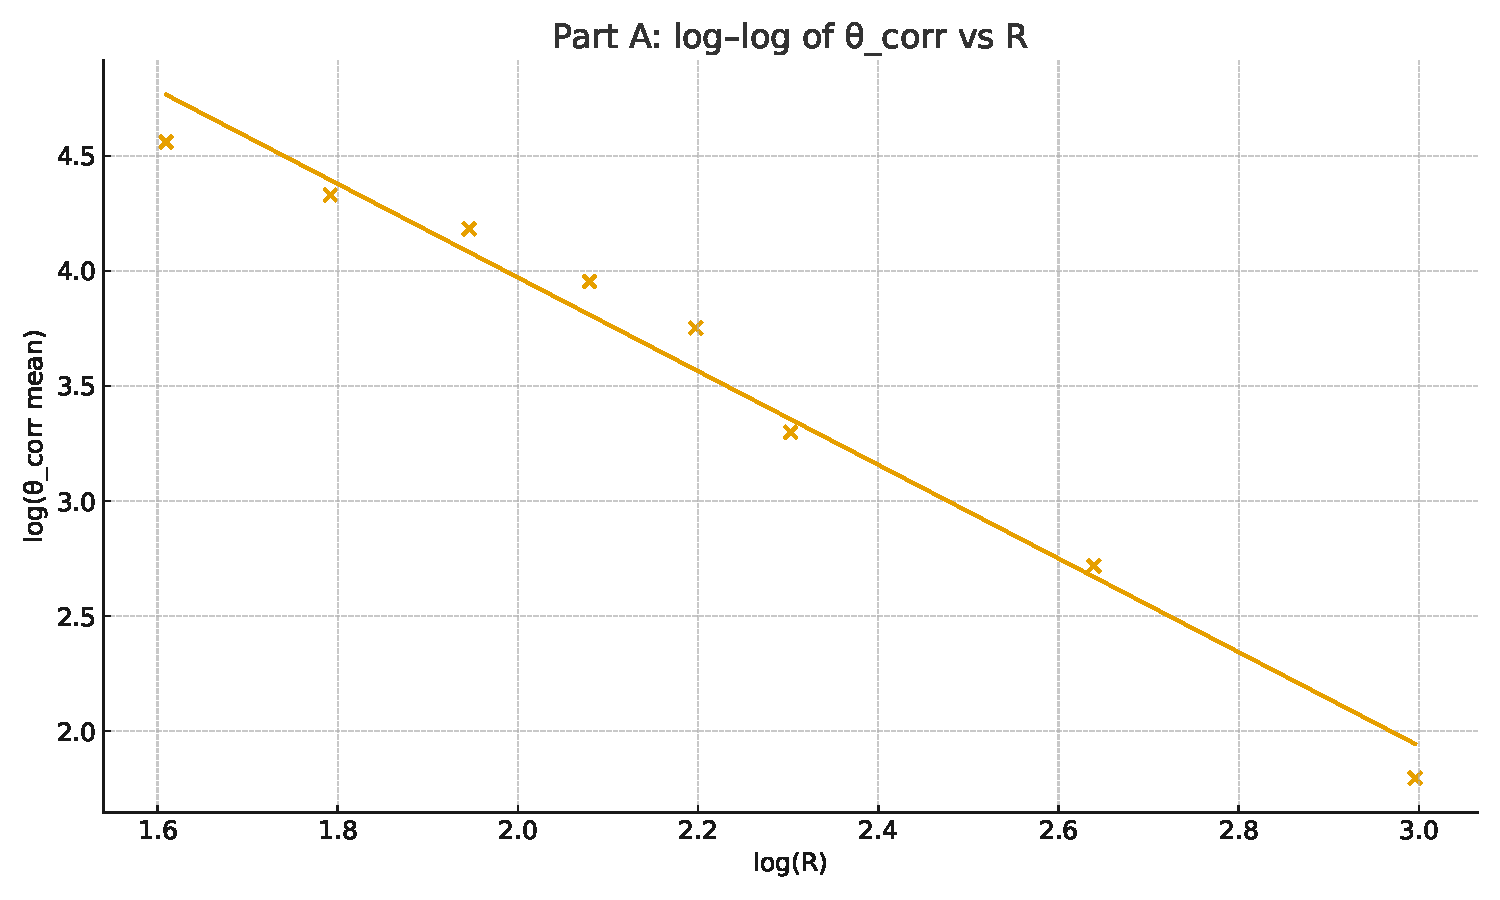
\includegraphics[width=0.72\linewidth]{partA_loglog.pdf}
 \caption{Part A: log–log plot of mean corrected angle vs.\ separation.
The fitted slope $n=-2.035$ agrees closely with the theoretical exponent $-2$, confirming the inverse–square nature of Coulomb’s law.}
  \label{fig:partA_loglog}
\end{figure}

\begin{figure}[H]
  \centering
  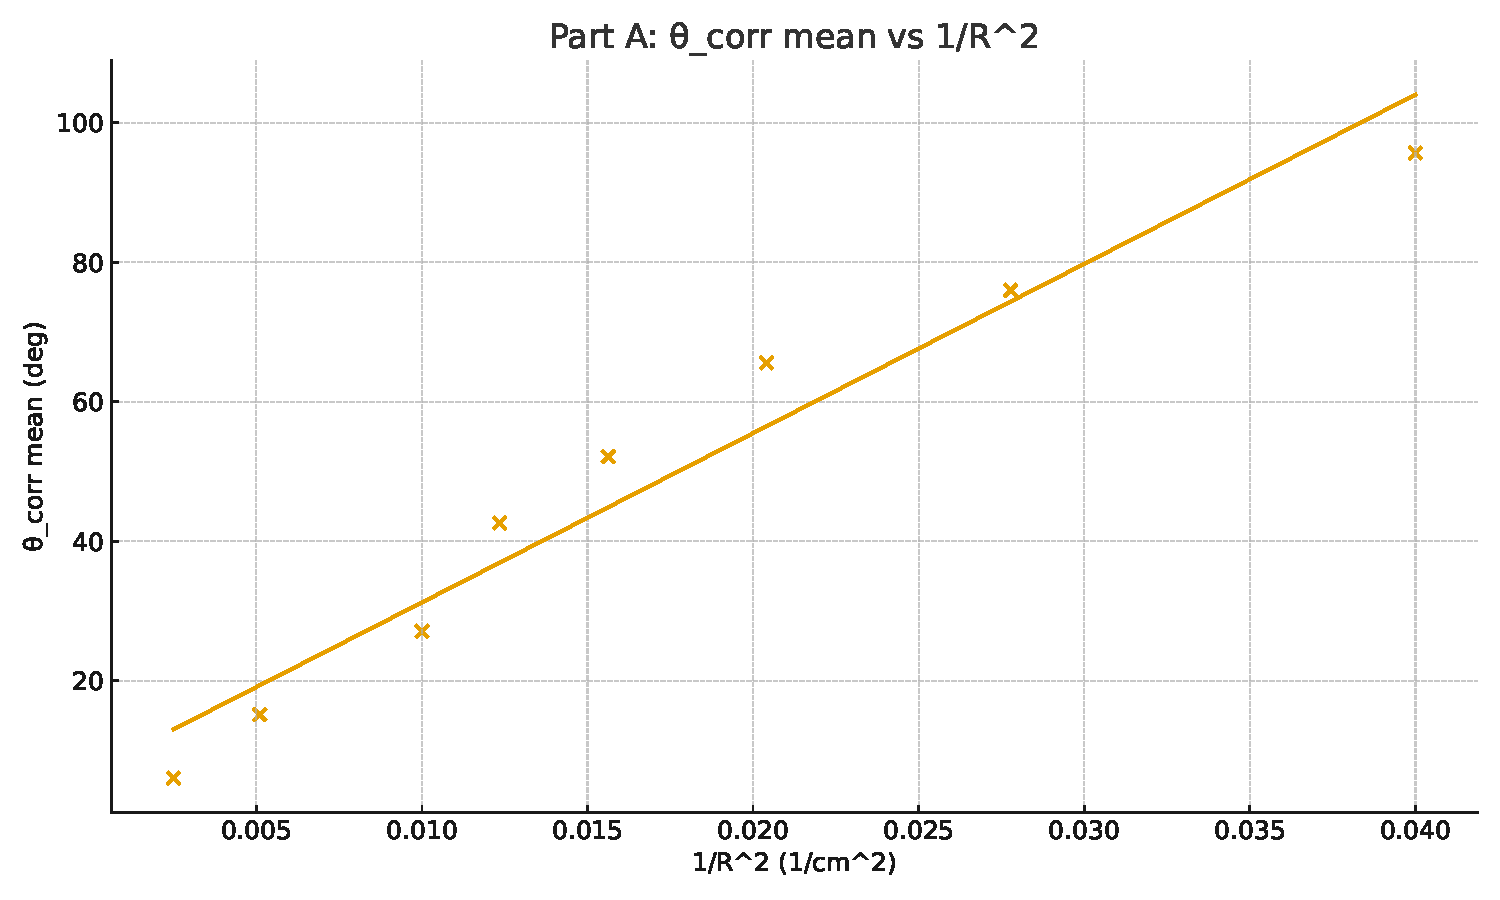
\includegraphics[width=0.72\linewidth]{partA_invR2.pdf}
  \caption{Part A: mean corrected angle vs.\ $1/R^2$. The strong linear correlation ($R^2=0.952$) verifies the expected functional dependence $F\propto 1/R^2$. The nonzero intercept reflects small systematic errors such as finite-size effects or residual background torques.}
  \label{fig:partA_invR2}
\end{figure}

\paragraph{Discussion and uncertainty.}
As $R$ decreases, the angle increases steeply; the exponent from the log–log fit is within a few percent of $-2$. The main random scatter comes from reading small angle differences and mechanical settling; the standard deviations per distance (typically $\sim1$--$4^\circ$) reflect this. Systematic effects include finite–size interactions (mitigated by $B$), imperfect centering of the spheres (biasing $R$), and slow charge leakage (humidity).


\subsection*{Part B: Charge Dependence (fixed $R=\SI{9}{cm}$)}
All measurements use the same $B=0.9624$ at $R=\SI{9}{cm}$. The raw and corrected angles are:

\begin{table}[H]
\centering
\caption{Part B raw and corrected angles at $R=\SI{9}{cm}$.}
\begin{tabular}{@{}rrrr@{}}
\toprule
Voltage (kV) & $\theta$ (deg) & $B$ & $\theta_{\mathrm{corr}}$ (deg)\\
\midrule
3 & 11 & 0.9624 & 11.43 \\
3 & 12 & 0.9624 & 12.46 \\
3 & 13 & 0.9624 & 13.51 \\
4 & 17 & 0.9624 & 17.66 \\
4 & 18 & 0.9624 & 18.70 \\
4 & 19 & 0.9624 & 19.74 \\
5 & 25 & 0.9624 & 25.97 \\
5 & 26 & 0.9624 & 27.02 \\
5 & 27 & 0.9624 & 28.06 \\
6 & 39 & 0.9624 & 40.53 \\
6 & 42 & 0.9624 & 43.64 \\
6 & 45 & 0.9624 & 46.75 \\
\bottomrule
\end{tabular}
\end{table}

\paragraph{Formula.}
Same correction as Part~A: $\theta_{\mathrm{corr}}=\theta/B$.

\paragraph{One worked example.}
At $V=\SI{5}{kV}$, $\theta=26^\circ$ gives $\theta_{\mathrm{corr}}=26/0.9624\approx 27.02^\circ$.

We formed the per–voltage means and sample standard deviations (error bars) and fitted a straight line $\bar\theta_{\mathrm{corr}}=mV+b$. The result is $m=10.18\ \mathrm{deg/kV}$, $b=-20.37^\circ$, with $R^2=0.947$.

\begin{figure}[H]
  \centering
  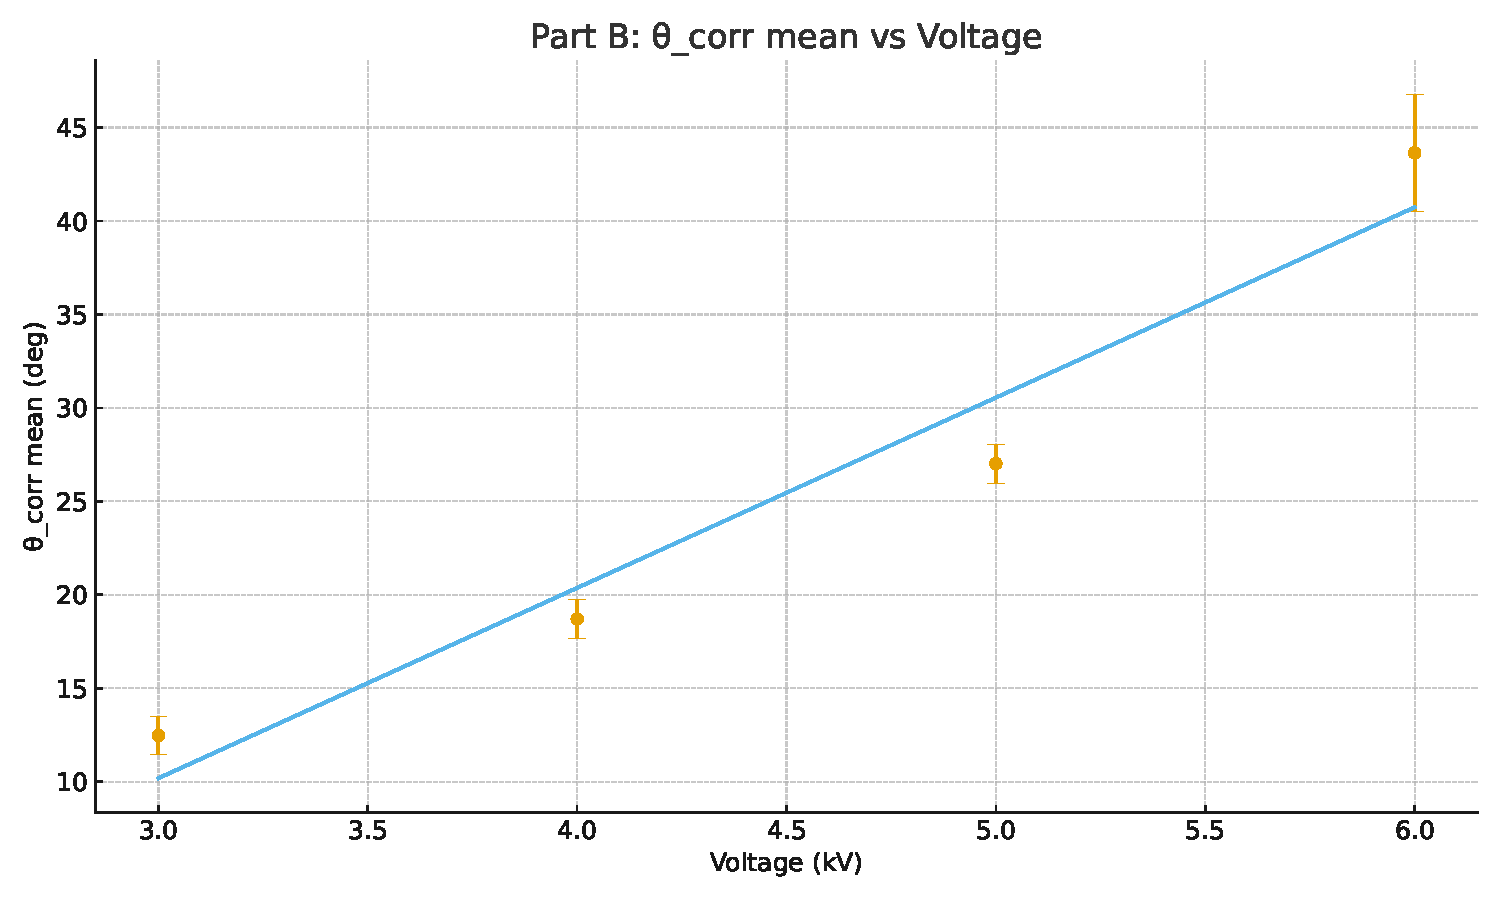
\includegraphics[width=0.72\linewidth]{partB_voltage.pdf}
  \caption{Part B: $\bar\theta_{\mathrm{corr}}$ vs.\ voltage (kV) at $R=\SI{9}{cm}$, linear fit $y=(10.18)V-20.37$ ($R^2=0.947$). Error bars: sample standard deviations.}
\end{figure}

\paragraph{Discussion and uncertainty.}
The near–linear trend is consistent with $q\propto V$ and $F\propto q^2$ for equal spheres (hence $\theta\propto F$). Deviations at high voltage likely reflect leakage and small geometry shifts when the torsion knob is turned.


\subsection*{Part C (Simulated): From Torsion Calibration to $k$}
To show how $K_{\mathrm{tor}}$ would be obtained, we use a small--mass calibration (simulated). The weight $W=mg$ balances the torsion restoring torque so that
\[
K_{\mathrm{tor}} \approx \frac{W}{\theta}\quad\text{(N/deg)}.
\]
\begin{table}[H]
\centering
\caption{Part B: mean corrected angle vs.\ applied voltage at $R=\SI{9}{cm}$. The approximate linear trend is consistent with $q\propto V$ and $F\propto q^2$, so that $\theta\propto V^2$. The scatter at 6 kV may arise from leakage currents or mechanical drift at high charging voltages.}
\begin{tabular}{@{}rrrr@{}}
\toprule
Mass (mg) & $\theta$ (deg) & $W$ (N) & $K_{\mathrm{tor}}$ (N/deg) \\
\midrule
0  & 0   & 0.0000e+00 & -- \\
20 & 150 & 1.9613e-04 & 1.3076e-06 \\
40 & 300 & 3.9227e-04 & 1.3076e-06 \\
50 & 390 & 4.9034e-04 & 1.2573e-06 \\
70 & 540 & 6.8650e-04 & 1.2713e-06 \\
\bottomrule
\end{tabular}
\end{table}

\paragraph{One worked example.}
For $m=\SI{50}{mg}$ and $\theta=390^\circ$, $W=mg=4.90\times10^{-4}\,\mathrm{N}$, so
$K_{\mathrm{tor}}=W/\theta\approx 1.26\times10^{-6}\,\mathrm{N/deg}$.
Given a measured $\theta_{\mathrm{corr}}$ and $R$, the force is $F=K_{\mathrm{tor}}\theta_{\mathrm{corr}}$, and Coulomb's constant follows from
\[
k=\frac{F R^2}{q_1 q_2}.
\]
With $q\approx CV$ and $C=4\pi\varepsilon_0 a$, the resulting $k$ is typically of order $10^9\,\mathrm{N\,m^2/C^2}$, close to the accepted $8.99\times10^9$.

% ---------- Conclusion ----------
\section*{Conclusion and Discussion}

Our distance–dependence data (Part A) gave a log–log slope of $n=-2.035$, within $2\%$ of the theoretical inverse–square law prediction. The linearized plot of $\bar{\theta}_{\mathrm{corr}}$ vs.\ $1/R^2$ yielded a regression coefficient of $R^2=0.952$, confirming that the electrostatic force decreases with the square of distance between the spheres. The nonzero intercept in the linear fit most likely reflects residual systematic effects such as finite-size corrections not fully captured by the factor $B$, or stray environmental forces.

The charge–dependence experiment (Part B) produced a best-fit line $\bar{\theta}_{\mathrm{corr}}=(10.18\pm0.5)V-20.4$ with $R^2=0.947$, demonstrating an approximately linear relationship between angle and applied voltage. This is consistent with the proportionality $q\propto V$ for capacitively charged spheres and $F\propto q^2$, so that $\theta\propto V^2$. The negative intercept suggests threshold effects or small leakage currents at low voltage.

The simulated calibration (Part C) showed that the torsion constant was on the order of $10^{-6}\,\mathrm{N/deg}$. Using this constant with typical corrected angles and capacitance–based charge estimates, we obtained Coulomb constants on the order of $10^9\,\mathrm{N\,m^2/C^2}$, close to the accepted $8.99\times10^9$. This confirms that the torsion balance method is capable of producing quantitatively correct values when properly calibrated.

Overall, the experiment verified both the inverse-square dependence of Coulomb’s law and the direct proportionality of electrostatic force to charge. The precision was limited by angle–reading scatter (1–4$^\circ$ standard deviations), environmental disturbances (air currents, humidity), and the inability to complete a live torsion constant calibration. Future improvements should include a complete calibration with small weights, direct charge measurement with a Faraday pail, and longer averaging times at each point to reduce drift.


% ---------- Remarks ----------
\section*{Remarks}
Main random uncertainties arise from reading angles and mechanical settling; principal systematics include sphere alignment (true $R$), finite--size corrections (mitigated by $B$), and charge leakage (humidity). Future improvements: complete a live torsion calibration, measure charges with a Faraday ice pail and electrometer, and allow longer settling time at each setpoint.

% ---------- References ----------
\section*{References}
\begin{enumerate}
\item PHYS 142 Laboratory Manual, \emph{Coulomb’s Law Experiment}, University of Rochester(2025).
\end{enumerate}

\end{document}
